\documentclass{article}

\usepackage[brazil]{babel}
\usepackage[T1]{fontenc}
\usepackage[a4paper, margin=1.5cm]{geometry}
\usepackage[colorlinks, urlcolor=blue, citecolor=red]{hyperref}
\usepackage[utf8]{inputenc}
\usepackage{graphicx, wrapfig}

\title{\textbf{Método de Monte Carlo para caminhos aleatórios}}
\author{Emmanuel Podestá Jr., Gustavo Zambonin\thanks{
        \texttt{\{emmanuel.podesta,gustavo.zambonin\}@grad.ufsc.br} \hfill
        \texttt{\href{https://github.com/zambonin/ufsc-ine5425}{src/}}
    } \\
    \small{Modelagem e Simulação (UFSC-INE5425)}
}
\date{}

\begin{document}

\maketitle

\section{Documentação}

Toda a documentação pode ser consultada junto ao código-fonte, acessível pelo
repositório referenciado neste documento (em inglês). Abaixo, uma breve
explanação das técnicas utilizadas para criar o programa será feita, dividida
pelos arquivos que compõem o projeto.

\subsection{\texttt{\_\_main\_\_.py}}

Responsável por executar código referente à inicialização do programa, visto
que este é distribuído com classes separadas. A janela para interface com o
usuário é criada, e após o término de sua execução, bibliotecas internas lidam
com a finalização do programa.

\subsection{\texttt{custom\_canvas.py}}

Apresenta uma classe pai representando as figuras criadas pela biblioteca de
gráficos, compatíveis com a interface escolhida, bem como três especializações
desta (uma para o gráfico do caminho percorrido, outra para o gráfico das
distâncias, e a final para a criação do histograma). A interatividade desses
gráficos também é adicionada nessa classe. Os dados necessários são obtidos a
partir da \emph{thread} que faz todas as computações.

\subsection{\texttt{monte\_carlo.py}}

Implementa uma \emph{thread} específica para a resolução dos cálculos
apresentados no problema, ou seja, geração de números pseudo-aleatórios,
emissão de sinais referentes ao progresso do cômputo para popular a barra de
progresso e transferir dados para as classes referentes à produção dos
gráficos, e avanço nas coordenadas $(x, y)$ de acordo com certo ângulo sorteado
anteriormente.  Caso não existisse barra de progresso, o isolamento destes
cálculos em uma especialização de \emph{thread} seria desnecessária.

\subsection{\texttt{qt\_window.py}}

Consiste da construção de janela personalizada para a finalidade do simulador,
concisa e discreta, com apenas um botão de controle, cuja função é inicializar
a \emph{thread} responsável pela simulação numérica, e dois parâmetros
modificáveis. Também lida com eventos de teclado e \emph{mouse} para controle
do programa e posicionamento dos elementos internos por meio de \emph{layouts},
e da janela em relação à resolução disponível no computador utilizado.

\begin{figure}[htbp]
    \centering
    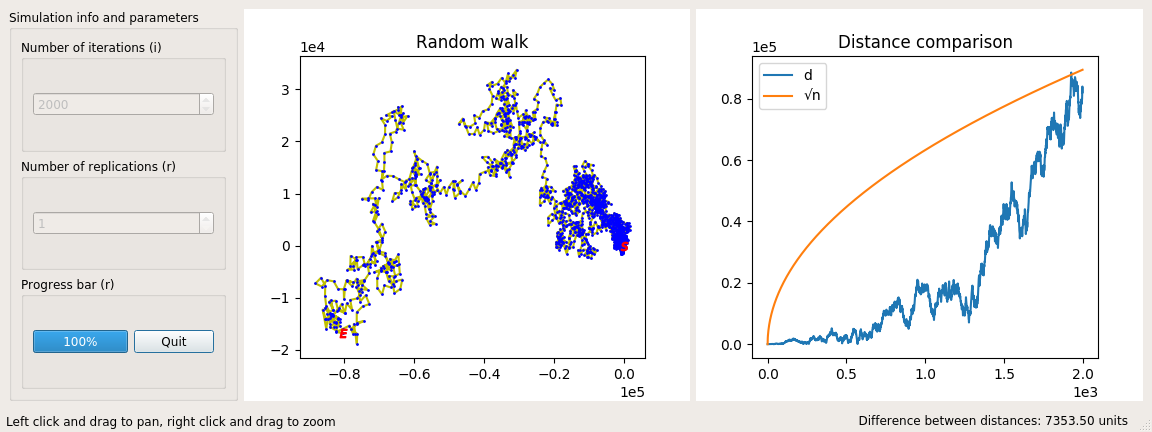
\includegraphics[scale=0.4]{example_run.png}
    \caption{Tela de resultados do programa se $r = 1$. Note que sua aparência
    pode mudar entre sistemas operacionais.}
\end{figure}

\section{Utilização}

\begin{wrapfigure}{r}{6cm}
    \centering
    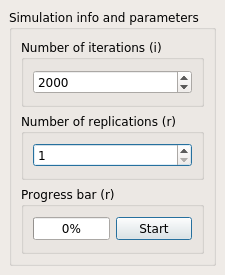
\includegraphics[scale=0.65]{program.png}
    \caption{Tela inicial do programa.}
\end{wrapfigure}

O simulador pode ser obtido a partir do repositório referenciado neste
documento, \href{https://github.com/zambonin/UFSC-INE5425/releases}{na seção de
downloads}. Após descompactá-lo, o usuário deve acessar a pasta criada e
executar o arquivo \texttt{drwalk.exe}. Os parâmetros podem ser configurados
com números no intervalo $[1, 2^{31} - 1]$, porém aconselha-se a utilização de
valores razoáveis, em virtude do desempenho da linguagem escolhida.
\vspace{2mm}

\noindent Ao acionar o botão para iniciar a simulação (ou apertar
\texttt{ENTER}), o usuário poderá acompanhar a computação a partir de uma
barra de progresso. Ao fim desta, se $r = 1$, dois gráficos serão mostrados:
o caminho aleatório feito a partir das $i$ iterações, bem como a distância
percorrida e esperada. Caso contrário, um histograma das diferenças entre as
distâncias será apresentado. Todos os gráficos são interativos: arrastar o
clique esquerdo do \emph{mouse} moverá o ponto de referência do gráfico, e
arrastar o clique direito proverá \emph{zoom}. O programa termina quando
\texttt{Esc} é acionado em qualquer momento de sua execução.

\end{document}
